\documentclass{article}
\usepackage[utf8]{inputenc}
\usepackage{graphicx}
\usepackage{float}
\usepackage{amsmath}

\title{Methods and Tools for Industrial Automation \\ First Project}
\author{M. Cardano - M. Cardellini - S. Lavaggi}
\date{\today}

\begin{document}

\maketitle

\section{Goal of the project}
In this project we were asked to build a controller able to adjust the movement of an autonomous vehicle in a way to reduce the error on the path to follow. Our goal was not to plan a path that the vehicle should follow, but instead, given a path, to build a controller able to bring the vehicle on the path. 

\section{Structure of the paper}
In Section 3 we give a small review of the models used to simulate a vehicle. We will start with a simple model and then build into one more complicated but that allows to better track the movement of the vehicle. The models presented are all taken from \cite{paper} which Prof. Sacile kindly assigned to us. In Section 4 we give an explanation of our controller and the code implemented in Matlab in order to achieve the result.

\section{Models for Vehicle Simulation}
\subsection{Geometric Bicycle Model}
\begin{figure}[H]
	\centering
    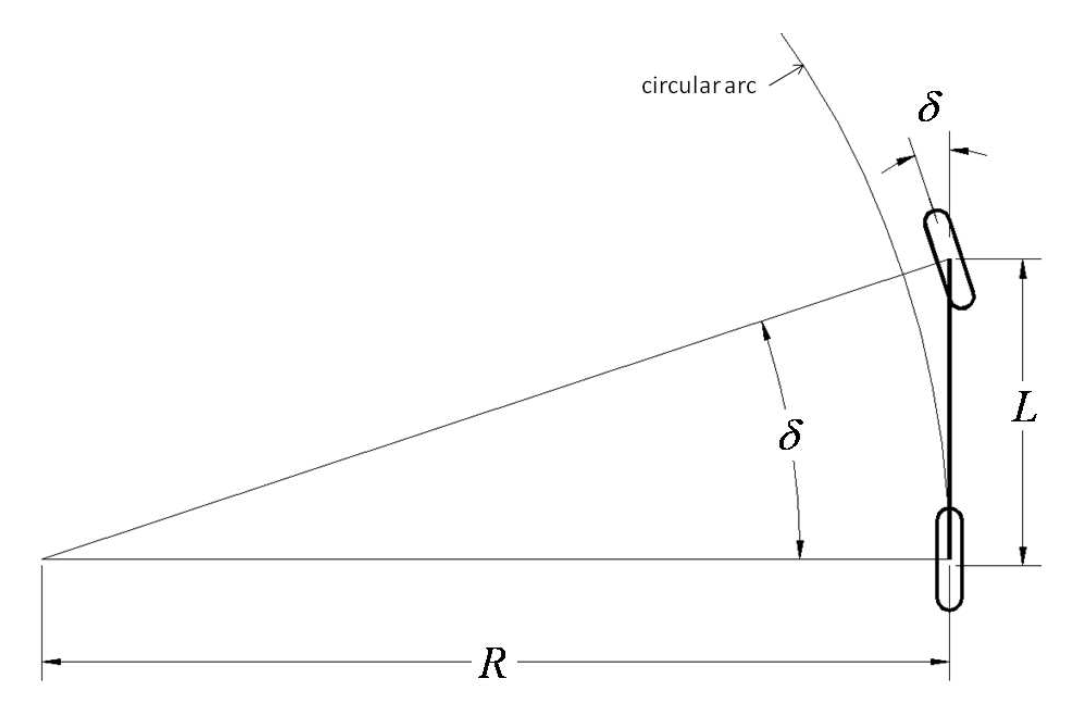
\includegraphics[width=200pt]{bicycle.png}
    \caption{Geometric Bicycle Model}
    \label{bicycle}
\end{figure}
A common semplification of a vehicle is the bicycle model which simplifies the four wheel car by combining the two front wheels together and the two rear wheels together to form a two wheeled model, like a bicycle. The second simplification is that the vehicle can only move on a plane. Figure \ref{bicycle} illustrates the model and the variables used to model it. \\ \\ The simple geometric relationship between the steering angle and the curvature that the rear axle will follow is 
\begin{equation}
	tan(\delta) = \frac{L}{R}
\end{equation}
where $\delta$ is the steering angle of the front wheel, $L$ is the distance between the front axle and the rear axle and $R$ is the radius of the circle that the rear axle will travel along at the given steering angle.

\subsection{Dynamic Bicycle Model}
It is clear that neglecting vehicle dynamics in the previous models has a negative impact on tracking performance as speeds are increased and path curvature varies. The dynamics of a car are very complicated and high fidelity models are very non-linear, discontinuous and computationally expensive.

\begin{figure}[H]
	\centering
    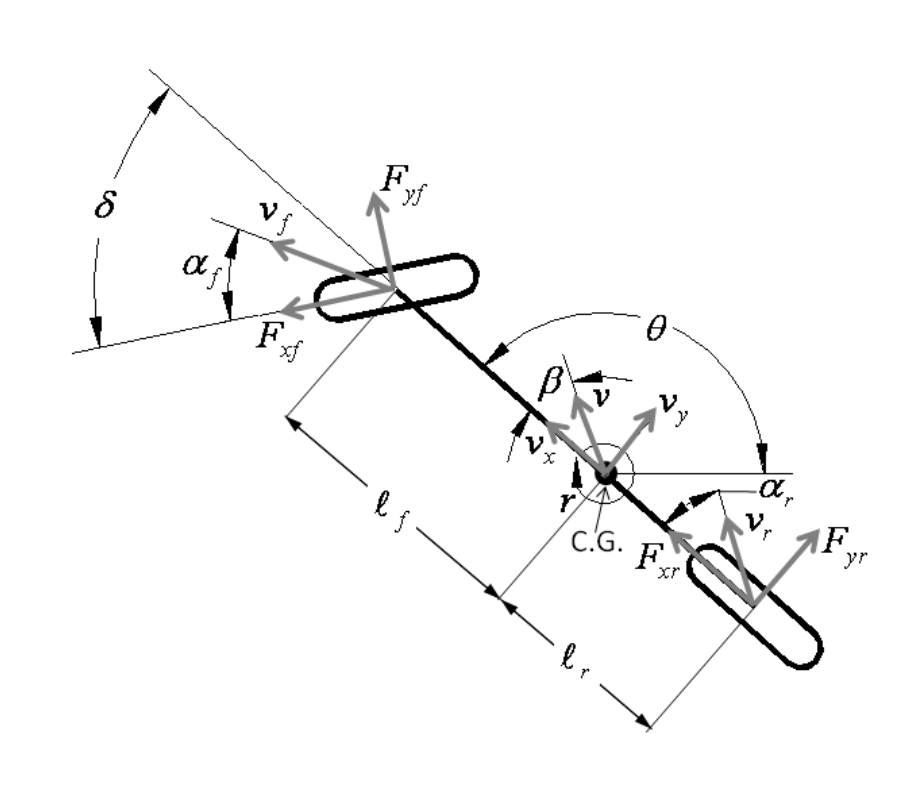
\includegraphics[width=200pt]{dynamic_bicycle}
    \caption{Dynamic Bicycle Model}
    \label{dynamic}
\end{figure}

The bicycle model introduced in the last section can be extended to include dynamics. Lateral forces on the vehicle are of primary concern as path tracking is an exercise in lateral control. For this section, longitudinal velocity is assumed to be controlled separately. Summing the lateral forces illustrated in Figure \ref{dynamic}, given vehicle mass m, yields
\begin{equation}
	F_{yf}cos(\delta) - F_{xf}sin(\delta) + F_{yr} = m(\dot{v}_y + v_xr)
\label{eq19}
\end{equation}
Considering only motion in the plane, a center of gravity C.G. along the center line of the vehicle, and yaw inertia Iz , balancing the yaw moments gives
\begin{equation}
	\ell_f(F_{yf}cos(\delta)) -\ell_r(F_{yr} - F_{xf}sin(\delta)) = I_z\dot{r}
\label{eq20}
\end{equation}
where $r$ is the angular rate about the yaw axis. The slip angles of the tires are given as
\begin{eqnarray}
\alpha_f &=& \tan^{-1}\left( \frac{v_y + \ell_f r}{v_x} \right) -\delta \\
\alpha_r &=& \tan^{-1}\left( \frac{v_y - \ell_r r}{v_x} \right)
\end{eqnarray}
Modelling the force generated by the wheels as linearly proportional to the slip angle, the lateral forces are defined as
\begin{eqnarray}
F_{yf} = - c_f\alpha_f \\
F_{yr} = - c_r\alpha_r
\label{eq21}
\label{forcesyfyr}
\end{eqnarray}
Where $c_f$ and $c_r$ are the proportional constants between the forces and the slip angle. Assuming a constant longitudinal velocity $\dot{v}_x = 0$, allows the simplification
\begin{equation}
	F_{xf} = 0
\label{eq22}
\end{equation}
\paragraph{Non Linear Model}
Substituting Eqs. \ref{eq21} and \ref{eq22} into Eqs. \ref{eq19} and \ref{eq20} and solving for $\dot{v}_y$ and $\dot{r}$
\begin{eqnarray}
	\dot{v}_y &=& \frac{-c_f\left[\tan^{-1}\left(\frac{v_y + \ell_f r}{v_x}\right) - \delta\right]\cos(\delta) - c_r \tan^{-1}\left(\frac{v_y - \ell_rr}{v_x}\right)}{m} - v_xr \\  
	\dot{r} &=& \frac{-\ell_fc_f\left[\tan^{-1}\left(\frac{v_y + \ell_f r}{v_x}\right) - \delta\right]\cos(\delta) + \ell_rc_r \tan^{-1}\left(\frac{v_y - \ell_rr}{v_x}\right)}{I_z} 
\end{eqnarray}
gives the dynamic bicycle model.

\paragraph{Linearized Model} To apply linear control methods to the dynamic bicycle model, the model myst be linearized. Applying small angle assumption to eqs 9 and 10 and writing it in state space form gives
\begin{equation}
 \begin{bmatrix} \dot{v}_y \\\\ \dot{r} \end{bmatrix}
 =
 \begin{bmatrix} \frac{-(c_f + c_r)}{mv_x} && \frac{\ell_rc_r - \ell_fc_f}{mv_x} - v_x \\\\ \frac{\ell_rc_r - \ell_fc_f}{I_zv_x} && \frac{-(\ell^2_fc_f + \ell^2_rc_r)}{I_zv_x}\end{bmatrix}
  \begin{bmatrix}v_x \\\\ r\end{bmatrix} + 
  \begin{bmatrix}
  	\frac{c_f}{m} \\\\ \frac{\ell_fc_f}{m}
  \end{bmatrix}  \delta
\end{equation}
\paragraph{Path coordinates} It is useful to express the dynamic bicycle model with respect to the path. 
\begin{figure}[H]
	\centering
    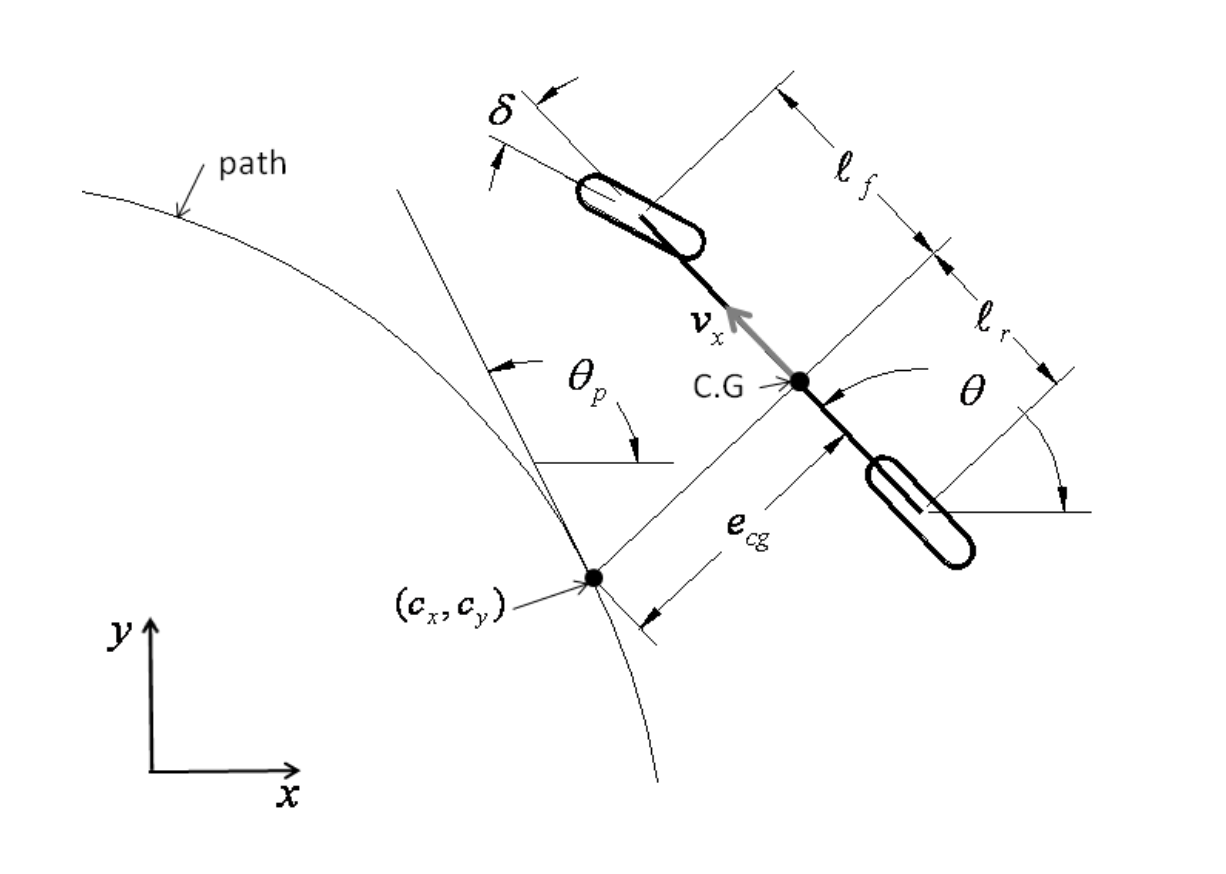
\includegraphics[width=200pt]{path}
    \caption{Dynamic Bicycle Model in path coordinates}
    \label{dynamic}
\end{figure}
Defining $\dot{e}_{cg}$ as the velocity of drift from the path and $\theta_e = \theta - \theta_p$ as the error of the angle and knowing that
\begin{equation}
	\dot{e}_{cg} = v_y + v_x\sin(\theta_e)
\end{equation}
we can write the state space model in tracking error variables as
\begin{eqnarray}
 \begin{bmatrix} 
 	\dot{e}_{cg} \\\\
 	\ddot{e}_{cg} \\\\
 	\dot{\theta_e} \\\\
 	\ddot{\theta_e} \\
 \end{bmatrix} &=& 
 \begin{bmatrix} 
 	0 & 1 & 0 & 0 \\\\
 	0 & \frac{-(c_f + c_r)}{mv_x} & \frac{c_f + c_r}{m} & \frac{\ell_fc_f - \ell_rc_r}{mv_x}\\\\
 	0 & 0 & 0 & 1 \\\\
 	0 & \frac{\ell_rc_r - \ell_fc_f}{I_zv_x} & \frac{\ell_fc_f - \ell_rc_r}{I_z} & \frac{-(\ell^2_fc_f + \ell^2_rc_r)}{I_zv_x}\\
 \end{bmatrix}
 \begin{bmatrix} 
 	{e}_{cg} \\\\
 	\dot{e}_{cg} \\\\
 	{\theta_e} \\\\
 	\dot{\theta_e} \\
 \end{bmatrix}\\ &+& \begin{bmatrix} 
 	0 \\\\
 	\frac{c_f}{m} \\\\
 	0 \\\\
 	\frac{\ell_fc_f}{I_z} \\
 \end{bmatrix} \delta
 + \begin{bmatrix} 
 	0 \\\\
 	\frac{\ell_rc_r - \ell_fc_f}{mv_x} - v_x \\\\
 	0 \\\\
 	\frac{-(\ell^2_fc_f + \ell^2_rc_r)}{I_zv_x} \\
 \end{bmatrix} r(s)
\end{eqnarray}

\section{Linear Quadratic Regulator}
\paragraph{Parameters.} The paper gave us all the parameters based on experiments:
\begin{eqnarray*}
	m &=& 1140 \\ 
	I_z &=& 1436.24\\ 
	\ell_f &=& 1.165 \\
	\ell_r &=& 1.165 \\
	c_f &=& 155494.663 \\
	c_r &=& 155494.663 \\
	v_x &=& 1.1765
\end{eqnarray*}
\paragraph{The state space}
The state matrix A becomes:
\begin{eqnarray}
 A &=& 
 \begin{bmatrix} 
 	0 & 1 & 0 & 0 \\
 	0 & -231.8722 & 272.7977 & 0\\
 	0 & 0 & 0 & 1 \\
 	0 & 0 & 0 & -249.7919\\
 \end{bmatrix}
 \end{eqnarray}
 The eigenvalues of the matrix A are:
 \begin{equation}
 	eig(A) = \begin{bmatrix} 
 	0 & -231.8722 & 0 & -249.7919 \\
 \end{bmatrix}^T \end{equation}
and so the system is not stable because of the two eigenvalues in zero.

\paragraph{Riccati's Equation.} To control the system we used an LQR. To minimize the cost function
$$ J = \sum_{\tau=0}^{N-1} (x_\tau^TQ_\tau x_\tau + u_\tau^TR_\tau u_\tau) + x^T_NQ_fx_N$$
that brings the error to zero by using the least possible control we used the Riccati's equation with the following parameters (as specified in the paper):
\begin{eqnarray*}
 Q &=& 
 \begin{bmatrix} 
 	5 & 0 & 0 & 0 \\
 	0 & 0 & 0 & 0\\
 	0 & 0 & 0 & 0 \\
 	0 & 0 & 0 & 0
 \end{bmatrix} \\\\
 R &=& 1 \\
 Q_f &=& Q \\
 \end{eqnarray*}
In this way we were able find the time-dependent matrix $K(\tau)$ to bring the tracking error to zero independently on the initial conditions:
\begin{eqnarray*}
	u_\tau &=& -K(\tau)x_\tau \\
	x_{\tau + 1} &=& A_dx_\tau + B_du_\tau;
\end{eqnarray*}
For example the following initial condition
$$x_0 = \begin{bmatrix} 
 	e_{cg} \\\\
 	\dot{e}_{cg} \\\\
 	\theta_e \\\\
 	\dot{\theta_e} \\
 \end{bmatrix} = \begin{bmatrix} 
 	2 \\\\
 	6.25 \\\\
 	-\frac{\pi}{2} \\\\
 	0 \\
 \end{bmatrix}$$
denotes a vehicle that is currently distant $2m$ from the path, moving away with a velocity of $6.25m/s$ perpendicular with the path. \\\\ 
We were able to bring the error to zero as seen in the following figure
\begin{figure}[H]
	\centering
    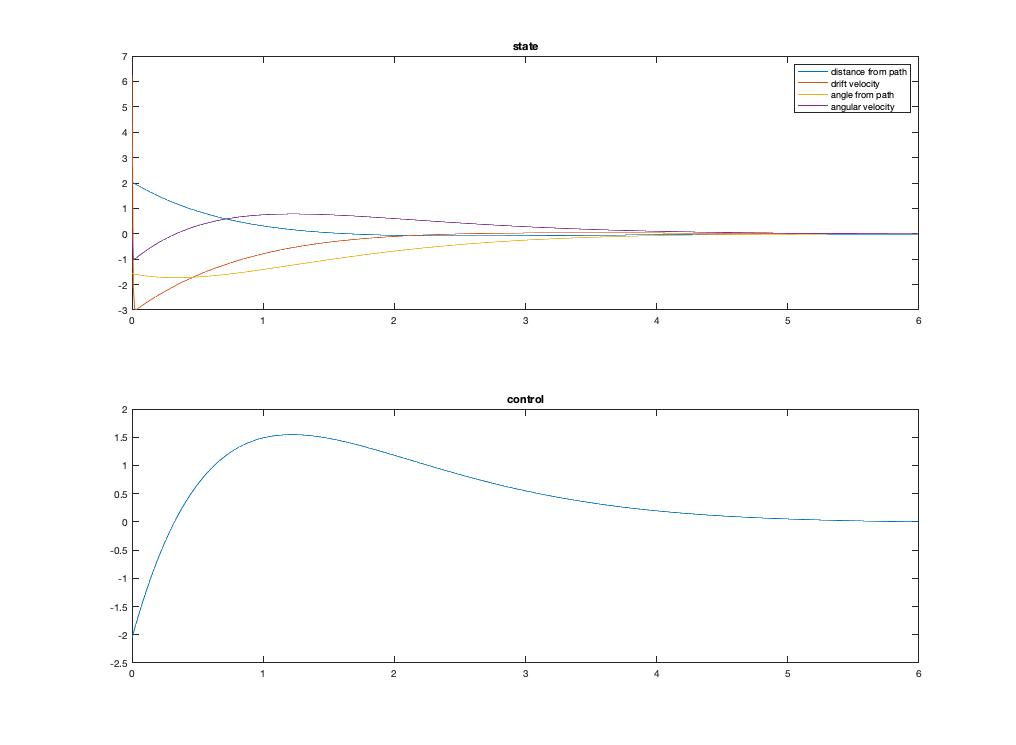
\includegraphics[width=350pt]{graph_new.jpg}
    \caption{State response to the proportional control $K(\tau)$}
    \label{dynamic}
\end{figure}



\bibliography{Citation}{}
\bibliographystyle{plain}

\end{document}
